\subsection{Stubfilter}

Im  Kapitel   \ref{sec:Protototypfilter}   wurde   gezeigt,   wie   durch  die
Entnormierung  eines  Prototypfilter  ein  konkretes  LC-Filter  dimensioniert
werden  kann.  Solche  LC-Filter  können   in   einem  weiten  Frequenzbereich
eingesetzt werden.  Jedoch wird bei realen konzentrierten Elementen (R,L,C) zu
höheren  Frequenzen hin  der  Einfluss  der  parasitären  Eigenschaften  immer
deutlicher, so dass  hohe  Anforderungen  an  die  Bauteilgüte gestellt werden
müssen.     Im    Bereich    von     einigen     \SI{100}{\mega\hertz}     bis
\SI{}{\giga\hertz}-Bereich   wird   es   daher   zunehmend  attraktiv,   statt
konzentrierten Kapazitäten und Induktivitäten verteilte Strukturen in Form von
Leitungen  zu  verwenden.\cite[p.~203]{ref:gustrau}   Man   spricht  dann  von
sogenannten Leitungsfiltern.

Es gibt  verschiedene Arten um Leitungsfilter zu realisieren. Eine Möglichkeit
der Realisierung  ist  das  Stubfilter.  Dieses  Filter  verwendet gleichlange
kurzgeschlossenen Leitungen (TLSC) und leerlaufende Leitungen(TLOC), welche an
einem   Ende   verbunden  und  am  anderen   Ende   entweder   kurzgeschlossen
oder offen gelassen werden. Diese sogenannten Stubs oder Stichleitungen werden
mit gleichlangen Verbindunsleitungen (TLIN) verbunden.

In  Abbildung \ref{fig:Stubfilter} ist ein solches Stubfilter zu sehen, welches aus
8 kurgeschlossenen Stubs (TLSC) besteht.

\begin{figure}[h!]
\centering
 	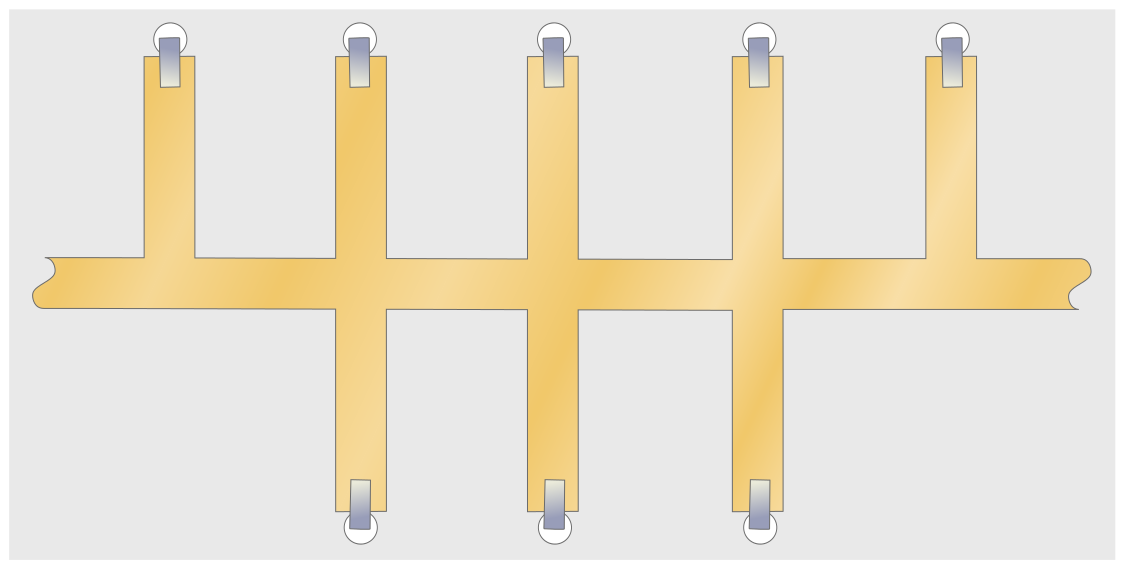
\includegraphics[width=\imagewidth]{images/Stripline_Stub_Filter}
 	\caption{Beispiel eines Stubfilters, Wikipedia \cite{ref:wikipedia:stripline}}
 	\label{fig:Stubfilter}
\end{figure}

Stubs  verhalten  sich bei hohen Frequenzen  wie  reaktive  Elemente(L,C)  und
ermöglichen  so  die  Realisierung  eines Mikrowellenfilters.  Für  Stubfilter
existiert  eine  geschlossene  Theorie  zur  Filtersynthese.  Dadurch muss ein
herrkömmliches Prototypfilter nur entnormiert und transformiert werden, um das
gewünschte   Stubfilter   mit   den  gewünschten  Eigenschaften  zu  erhalten.

